\documentclass{sig-alt-release2}
\usepackage{url}
\usepackage{color}
\usepackage{graphics,graphicx}

\usepackage{epsfig}
\usepackage{epstopdf}

\usepackage{colortbl}
\usepackage{multirow}
\usepackage{booktabs}
\usepackage{ifthen}  

\begin{document}
\newcommand{\todo}[1]{\textcolor{red}{#1}}
\def\newblock{\hskip .11em plus .33em minus .07em}

\conferenceinfo{DIM3} {2012, Glasgow, UK} 
\CopyrightYear{2012}
\clubpenalty=10000
\widowpenalty = 10000

\title{{iHero Specification}}

\numberofauthors{4}
\author{
\alignauthor 
Gary Blackwood \textit{0906796b}\\
Ian Scott \textit{0901475s}\\
John Dennis \textit{0907383d}\\
Paul Moore \textit{0901723m}\\
\affaddr{Fairweathers Kitchen}\\
\affaddr{DIM3}\\
}
\maketitle

\begin{abstract}
iHero is a new social media app that allows the general public to submit reports of incidents and disasters at their current location. Emergency service personnel will then be able to view the reports as submitted by the public. The idea is that an event will only be submitted once by the first user, and other users can vote up the credibility of the event and comment on the event to provide more detail.

The idea is that we are collating all the data in one place - as opposed to Emergency Services having to trawl through Twitter feeds and Facebook pages etc. It is in no way designed to replace calling the emergency services direct, but instead as a tool to aid them.
\end{abstract}

\section{Aim of Application}
iHero is a web application that will allow users to upload reports of incidents that occur in the real world. The main aim of this service is to provide information about incidents in a clear and concise way that can be used by emergency services. To sort the most important reports, users can give a rating of how serious the incident is when they submit it. This combined with allowing all users to vote submissions up or down should filter the most urgent incidents to the top of the list.

The required functionality of the application is:
\begin{itemize}
\item  Allow users to submit reports including a title/description, location and seriousness rating
\item  List recent incident reports and allow them to be voted up or down
\item  Mark the locations of the events on a map
\end{itemize}

It would also be desirable to :

\begin{itemize}
\item  Allow users to upload photos and videos with their submissions
\item  If the submission is made from a mobile device, pull the GPS location from it
\item "Did you mean this fire on xyz street?" feature to prevent many reports of the same incident
\end{itemize}

It is our goal to implement all the required functionality and as much of the desired as possible. The main constraint on this project is time and resources. We have limited time to implement the system and as a team of four people we feel the functionality is reasonably complex.

The finished application should also meet a number of non functional requirements. The website should be easily usable, we will do this by making a simple, clean client interface that emphasizes recognition over recall. It must also be reliable as the data we are receiving could potentially be very important. It is our aim to optimize the website for mobile devices because this will be where most of the incident reports come from. Doing this also allows the emergency services to locate incidents close to them when they are out and about.

\section{Client Interface}
Our interface must be minimal and clean. We provide our brand logo in the customary top left position to provide feedback to the user that they have arrived at the correct location (Label 1). The users may be in a state of shock or distress when using our system. As can be seen, from the wireframe below of the main screen, we ask for minimal amounts of required field data (Labels 3 through 5). Simply the event or disaster title, the exact location and a judgement of the seriousness rating. If using a mobile phone we will record geolocation data about the position the user is currently at but provide the user with a section to give more precise detail. We think this is enough data to allow other users to be able to verify an event. We provide a button to allow more data to be input should the user wish to give us more if the circumstances and surroundings should permit them to.

If the user opts to input more information the form will expand and allow them to upload a picture, video, extra details including the time of the incident, a box to give more details and also a tags field to aid searches.

The emergency services have a different view, accessible by the button labelled “Emergency Services Login” (Label 6) This will provide a listing of all the incidents and events, sortable on different categories. Emergency services will have the right to delete rogue information that they know to be untrue or exaggerated.

This easy, appealing and simple user interface allows the user to quickly fill out the emergency report and submit it to the iHero system - no complicated forms, a few select number of fields, and all in one page.

\begin{center}
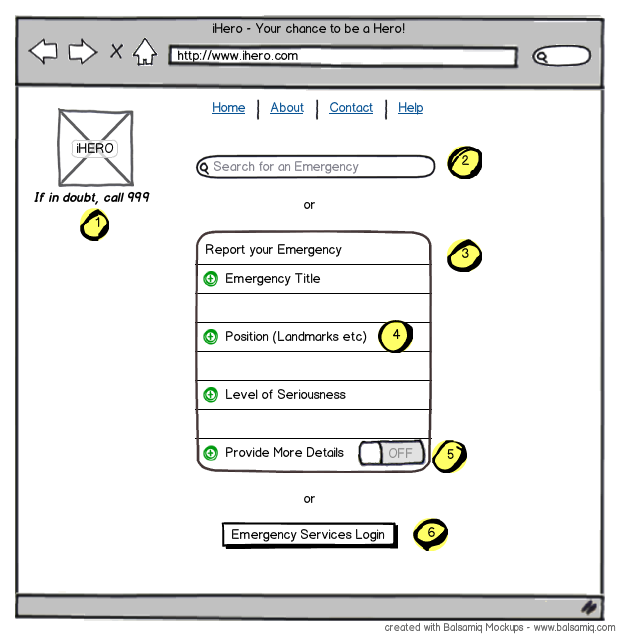
\includegraphics[scale=0.4]{img/1.png}
\end{center}

\subsection{Technologies}

\subsection{HTML}
It is anticipated we will use HTML5 or XHTML for this project. Using HTML5 brings us to the forefront of technology and provides us with the most up to date features for web based applications - however not all browsers can support this yet. This is where XHTML can be used for backwards compatibility, however this is more complex than basic HTML.

\subsection{CSS (Twitter Bootstrap)}
We plan to make use of the Twitter Bootstrap CSS framework to give a clean, familiar styling to our user interface. Using CSS (Cascading Style Sheets) is good programming practice as it removes all styling from the HTML code. This means that the style can change without having to edit the content, and vice versa. This seperates out concerns, as the style and content are independent of each other.

\subsection{jQuery and JavaScript}
We will also use jQuery to provide active content to our site, such as expanding the more details field if the user wishes to do so.

\newpage
\section{Application Architecture}

\begin{center}
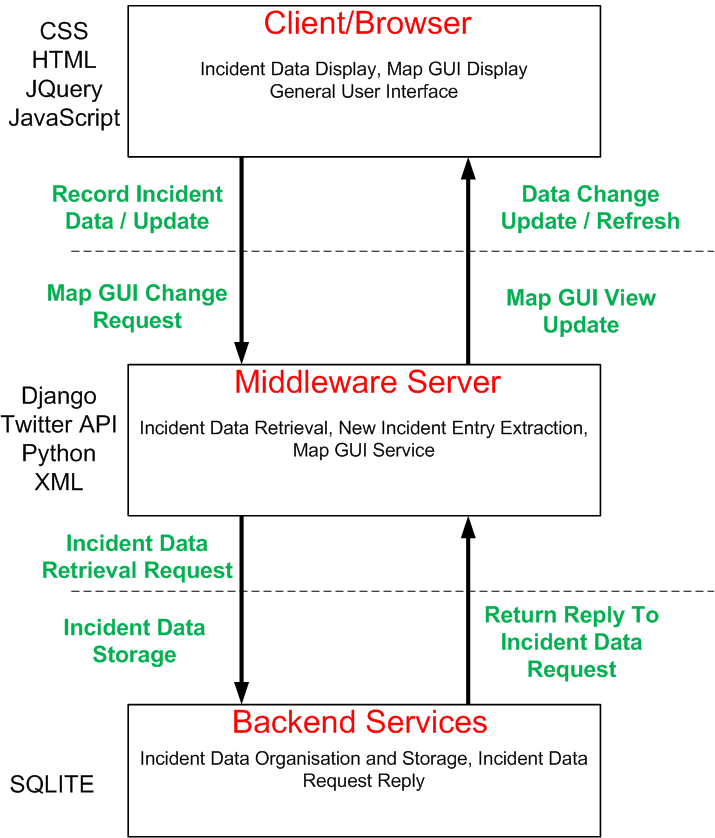
\includegraphics[scale=0.3]{img/2.png}
\end{center}

\subsection{Client/Browser}

\begin{itemize}
\item    Provides the interface for users to report an incident.
\item    Presents already reported incidents to the user.
\begin{itemize}
\item        Time.
\item        Location.
\item            Also presented in a map view.
\item        Description.
\end{itemize}
\item    Presents data in a structured and organised way using CSS.
\end{itemize}

\subsection{Middleware}

\begin{itemize}
\item    Acts as a receiver of user incident data entries from the Client Tier.
\begin{itemize}
\item        Passes this data on to the Backend Server (Database).
\end{itemize}
\item    Receives queries from the Client tier.
\begin{itemize}
\item        Extracts required data from the Backend server in response to these queries.
\end{itemize}
\end{itemize}

\subsection{Backend}


\begin{itemize}
\item    Provides the storage of incident data using the SQLITE database.
\item    Replies to data queries passed on by the Middleware Server.
\end{itemize}

\subsection{Data Flow}

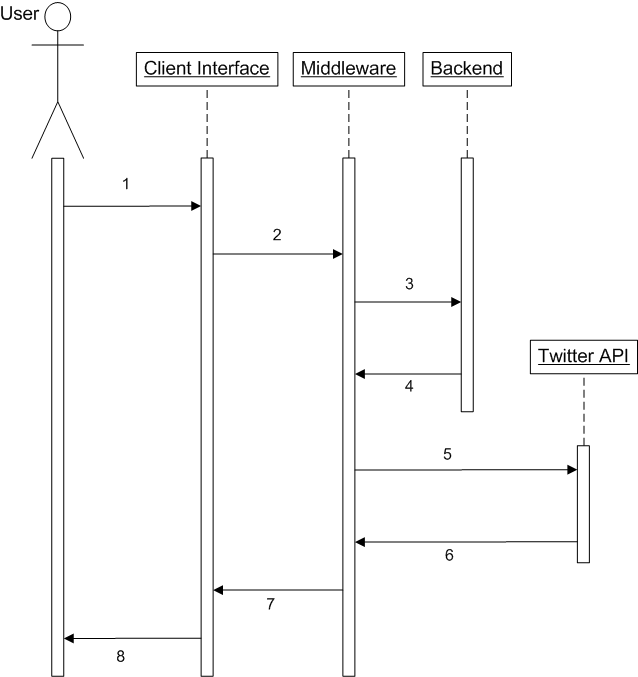
\includegraphics[scale=0.3]{img/3.png}

\begin{enumerate}
\item    User reports an incident, entering the time, location and description of the incident.
\item    Client Tier sends data of reported incident, or request for user to view another incident.
\item    Middleware Server communicates this query to the database in the Backend services and awaits a reply, or requests for new incident data to be stored in the database.
\item    Backend Services records new data and updates the database. Returns a refreshed state for the Middleware to provide to the Client Tier.
\item    Middleware provides new data to Twitter in the form of a tweet.
\item    Twitter API returns results of any queries from the Client Tier via Middleware.
\item    Middleware returns refreshed data back to the Client.
\item    Client displays up-to-date reflection of incident data.
\end{enumerate}

\subsection{Data Model}

\begin{center}
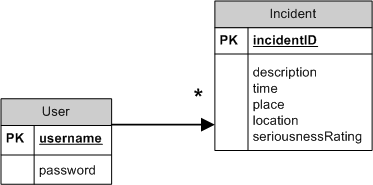
\includegraphics[scale=0.4]{img/4.png}
\end{center}

\begin{itemize}
\item    User profiles can be obtained from the Twitter service provided
\item    Users have their username and passwords stored
\item    Users have 0-many incidents
\item    Incidents have only one user, and have the following attributes: description, time, location, seriousness rating.
\end{itemize}


\section{Message Parsing}
\begin{itemize}

\item	On the architecture diagram, Identify and label the main messages that will be parsed through the application.
\item	or alternatively (and preferably) include sequence diagrams to denote the sequence of communications parse between clients and servers.
\item	Describe the messages that are parsed back and forth through the application.
\item	For the main transactions - describe the payload of the messages 
\item	i.e. What are the contents of the messages? i.e. include sample XML, XHTML, JSON, etc of one or two messages.
\item	What is the format of the messages? 
\item	Why this format? 
\item	What other formats could be used, what are the advantages and disadvantages of these other formats?
\end{itemize}



\section{Design Revision / Feedback}
{\bf For the Implementation Report Only:}
\begin{itemize}
\item	include a summary of the feedback given (or refer to specific comments from the feedback) 
\item	comment on how you have revised the design (if at all) according to the comments received 
\item	how has the feedback helped, and has this process been helpful.
\end{itemize}

\section{Implementation Notes}
{\bf For the Implementation Report Only:}

\begin{itemize}
\item Views - What are the main views that you have implemented and what do they do?
\item URL Mapping Schema - what is your URL mapping and schema?
\item External Services  - what external services does your application include and what handlers did you include?
\item	Functionality Checklist (which functionality is completed)
\item	Known Issues (what kind of works, what kind of errors to do you get)
\item What technologies have been used and are required for the application. Include a list or table of all the technologies, standards, and protocols that will be required.
\end{itemize}

\section{Reflective Summary}
{\bf For the Implementation Report Only:}
\begin{itemize}
\item	What have you learnt through the process of development? 
\item	How did the application of frameworks help or hinder your progress? 
\item	What problems did you encounter? 
\item	What were your major achievements?
\end{itemize}

\section{Summary and Future Work}
\begin{itemize}
\item	Summary of application and its current state.
\item	Include a list or table of all the technologies, standards, and protocols that will be required.
\item	What are the limitations?
\item Plans for future development
\end{itemize}

\section{Acknowledgements}
Our thanks to the lecturers and demonstrators for their comments and suggestions. And our thanks to the peer reviewers for their feedback.
Be sincere and be specific about how others have helped your group.

\bibliographystyle{abbrv}
\bibliography{sig-proc}

\end{document}
